\documentclass[11pt,a4paper]{article}
\usepackage[T1]{fontenc}
\usepackage[utf8]{inputenc}
\usepackage{mathptmx}
\usepackage[a4paper,margin=2.5cm]{geometry}
\usepackage{amsmath,amsthm}
\usepackage{graphicx}
\usepackage{booktabs}
\usepackage{enumitem}
\usepackage[section]{placeins}
\usepackage[font=small,labelfont=bf,labelsep=period]{caption}
\usepackage[hidelinks]{hyperref}
\graphicspath{{figures/}}
\setlength{\parskip}{3pt}
\setlength{\emergencystretch}{1.5em}
\setcounter{secnumdepth}{2}
\renewcommand{\topfraction}{0.9}
\renewcommand{\bottomfraction}{0.8}
\renewcommand{\textfraction}{0.07}
\renewcommand{\floatpagefraction}{0.75}
\renewcommand{\thesection}{\arabic{section}.}
\renewcommand{\thesubsection}{\arabic{section}.\arabic{subsection}.}

\newtheorem{theorem}{Theorem}
\newtheorem{remark}{Remark}
\newcommand{\bv}[1]{\mathbf{#1}}
\newcommand{\Jm}{\boldsymbol{\mathcal{J}}}

\begin{document}

\begin{center}
{\LARGE\bfseries Flatness-Based and Passivity-Based Control with Adaptive RBF Neural Compensation of a 2~MW Direct-Drive PMSG Wind Energy Conversion System\par}
\vspace{12pt}
{\large Said Regani, Manal Messadi and Karim Kemih\,*\par}
\vspace{6pt}
{\small L2EI Laboratory, Jijel University, BP 98, Ouled Aissa, Jijel 18000, Algeria;\\
said.regani@univ-jijel.dz (S.R.); manal.messadi@univ-jijel.dz (M.M.)\\
* Correspondence: karim\_kemih@univ-jijel.dz\par}
\end{center}

\vspace{6pt}
\noindent\textbf{Abstract:} This paper proposes a nonlinear control scheme with adaptive radial basis function (RBF)
neural compensation for a 2~MW direct-drive wind energy conversion system based on a permanent magnet
synchronous generator (PMSG) connected to the grid through a back-to-back converter and an $L$ filter.
First, a complete model of the system, from the wind to the grid, is established in the receptor
convention, and its signs are verified by an exact power balance. Subsequently, the rotor speed and the
energy stored in the DC link and in the filter are used as flat outputs of the two outer loops, and the
currents of both converters are controlled by passivity-based control (PBC), whose convergence is proved
with a storage function. To further enhance the speed tracking, an RBF network is introduced as a
complementary compensation of the aerodynamic-torque and parameter uncertainty, without retuning the
nominal gains. A Lyapunov-based adaptation law with $\sigma$-modification guarantees the uniform
ultimate boundedness of the speed error and of the network weights. The scheme is evaluated with step
and turbulent wind, parameter mismatch, a 50\,\% grid voltage dip, sensor noise and grid voltage
harmonics. Simulation results show that all the controlled variables track their references, that the
DC-link voltage remains within 0.8\,\% of its reference outside the dip, that the grid-current
distortion stays below 4\,\%, and that the neural compensation reduces the integral absolute speed error
by 26.5 to 44.8\,\% with the same captured energy.

\vspace{4pt}
\noindent\textbf{Keywords:} wind energy conversion systems; direct-drive PMSG; differential flatness;
passivity-based control; adaptive RBF neural network; back-to-back converter

%=====================================================================
\section{Introduction}
The increasing demand for clean energy and the need to reduce greenhouse gas emissions have made wind
energy one of the main sources of the transition towards low-carbon electricity generation.
Barthelmie and Pryor~\cite{barthelmie2021} discussed the contribution of wind energy to climate-change
mitigation, and the reports of the International Energy Agency~\cite{iea2024} and of the Global Wind
Energy Council~\cite{gwec2024} show the continuous growth of the installed capacity. This growth is
accompanied by larger turbines and by stricter requirements on the quality of the injected power.

Among the generator technologies used in variable-speed wind turbines, the direct-drive permanent
magnet synchronous generator (PMSG) has become an important solution. Polinder et al.~\cite{polinder2013}
reviewed the trends in wind turbine generator systems and showed that removing the gearbox reduces
maintenance and mechanical losses. Yaramasu et al.~\cite{yaramasu2015} and Wu et al.~\cite{wu2011}
described the full-scale back-to-back converter of these turbines: the machine-side converter (MSC)
controls the generator torque to track the maximum power point, and the grid-side converter (GSC)
regulates the DC-link voltage and injects the power into the grid. Since the whole power flows through
the converter, the generator is fully decoupled from the grid. Rol\'an et al.~\cite{rolan2009} and
Hasan and Shatil~\cite{hasan2021} presented the modeling and the design of grid-connected PMSG wind
turbines, which provide the data used in the present study.

These control tasks are usually performed by cascaded proportional-integral (PI) loops in rotating
reference frames. Chinchilla et al.~\cite{chinchilla2006} applied this vector control to permanent-magnet
generators connected to the grid, and Yazdani and Iravani~\cite{yazdani2010} and Blaabjerg et
al.~\cite{blaabjerg2006} detailed the modeling, the current control and the grid synchronization of
voltage-sourced converters. The PI loops are simple and robust, but they are tuned on a linearized model
and do not use the nonlinear structure of the system.

Considerable research has therefore been devoted to nonlinear control of wind energy conversion systems.
Mechter et al.\ proposed a sliding mode control with an exponential reaching law~\cite{mechter2015} and a
backstepping control for low wind speeds~\cite{mechter2016}. For the PMSG, Messadi et al.~\cite{messadi2015}
developed a predictive control of a chaotic PMSG in a wind turbine, Yang et al.~\cite{yang2021} designed a
fuzzy state-feedback control of a fractional-order direct-drive PMSG with uncertain parameters, and
Benabdeeseelam et al.~\cite{benabdeeseelam2025} proposed a chattering-free terminal sliding mode control
for a chaotic PMSG in an offshore wind turbine. Among the model-based methods, differential
flatness~\cite{fliess1995} computes the control directly from the desired trajectory of a flat output.
Aimene et al.~\cite{aimene2022} compared flatness-based and field-oriented control of a grid-connected
PMSG wind energy conversion system, and Thounthong et al.~\cite{thounthong2010} showed that, with the
stored energy as flat output, the DC-bus dynamics become a linear power balance. Passivity-based control
(PBC)~\cite{ortega1998,ortega2002} shapes the energy of the closed loop and keeps the workless coupling
terms of electrical machines, which makes it well suited to the current loops of the converters.

Learning-based approximators have also been exploited to handle the uncertainty of wind turbine models.
RBF networks are universal approximators~\cite{park1991}, and their weights can be adapted online with a
Lyapunov-based law~\cite{lewis1999}. Li et al.~\cite{li2024} introduced an RBF neural network-based global
fast terminal sliding mode control for a fully controlled doubly-fed induction generator, Dardabi et al.~\cite{dardabi2024}
used artificial neural networks to enhance the control of doubly-fed induction generators in the presence
of real wind profiles, and
Bounar et al.~\cite{bounar2025} proposed a disturbance-observer-based finite-time adaptive neural control
of a doubly-fed induction generator wind turbine. In our previous work~\cite{regani2026}, a nonlinear state-feedback controller was
combined with an adaptive artificial neural network that compensates the residual tracking error of a
doubly-fed induction generator; that study did not consider measurement noise or grid disturbances.

These studies show that nonlinear, adaptive and neural methods can improve the performance of wind
energy conversion systems. However, the existing works generally address one converter or one loop, and
the flatness-based and passivity-based methods use a model whose weak point is the aerodynamic torque,
which is not measured, and the generator parameters, which change with temperature and saturation. In
particular, increasing the gains of the speed loop is not an appropriate way to reduce the effect of
this uncertainty, because the speed loop multiplies the measurement noise by the large inertia of the
turbine. A control framework that combines flatness for the outer loops, PBC for the current loops of
both converters and an adaptive neural compensation of the aerodynamic uncertainty, and that is
evaluated under realistic measurements and grid disturbances, remains less explored.

Motivated by this gap, the present study proposes a flatness-based and passivity-based control with
adaptive RBF neural compensation for a 2~MW direct-drive PMSG wind energy conversion system. The neural
network does not replace the nominal controller; it adds a compensation term to the flat speed law, and
the nominal gains are kept unchanged. The main contributions of this work are summarized as follows:
\begin{itemize}[leftmargin=*,itemsep=2pt]
\item \textbf{Complete and verified model:} the system is modeled from the wind to the grid in the
receptor convention, and an exact power balance verifies the sign of every term of the model.
\item \textbf{Flatness-based outer loops:} the rotor speed and the energy stored in the DC link and in the
filter are used as flat outputs, so that the DC-link dynamics become a linear power balance.
\item \textbf{Passivity-based current loops:} the currents of both converters are controlled by PBC, and
their convergence is proved with a storage function and Barbalat's lemma.
\item \textbf{Adaptive RBF compensation:} an RBF network learns online the aerodynamic-torque and parameter
uncertainty with a Lyapunov-based law with $\sigma$-modification, and the uniform ultimate boundedness of
the speed error and of the weights is established.
\item \textbf{Realistic numerical validation:} the control is evaluated with the same nominal gains without
and with the network, under step and turbulent wind, parameter mismatch, sensor noise, grid voltage
harmonics and a 50\,\% voltage dip.
\end{itemize}

The remainder of this paper is organized as follows. Section~2 presents the mathematical modeling of the
PMSG wind energy conversion system. Section~3 describes the proposed flatness-based and passivity-based
control and its stability analysis. Section~4 presents the adaptive RBF compensation and the
corresponding uniform-ultimate-boundedness analysis. Section~5 presents the numerical simulations and
discusses the results. Finally, Section~6 concludes the paper and outlines directions for future work.

%=====================================================================
\section{Mathematical Modeling of the PMSG Wind Energy Conversion System}
The studied system is shown in Figure~\ref{fig:system}. The turbine drives the PMSG directly; the MSC
rectifies the generator voltages, the DC link decouples the two converters, and the GSC injects the
power into the 690~V, 50~Hz grid through an $L$ filter. The parameters of the system are given in
Table~\ref{tab:param}.

\begin{figure}[!htb]
\centering
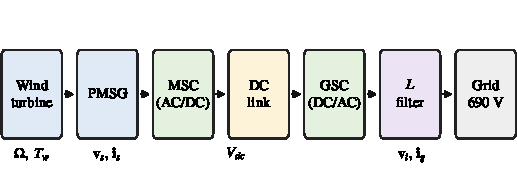
\includegraphics[width=0.75\textwidth]{system.pdf}
\caption{Direct-drive PMSG wind energy conversion system with a back-to-back converter.}
\label{fig:system}
\end{figure}

\subsection{Wind Turbine Aerodynamic Modeling}
The power captured by the rotor and the tip-speed ratio are~\cite{heier2014,aimene2022}
\begin{equation}
P_w = \tfrac{1}{2}\rho\pi R^2 C_p(\lambda,\beta)\,v^3,\qquad \lambda=\frac{\Omega R}{v},
\label{eq:pw}
\end{equation}
where $\rho$ is the air density, $R$ the rotor radius, $v$ the wind speed, $\Omega$ the rotor speed and
$\beta$ the pitch angle. The power coefficient is
\begin{equation}
C_p = 0.5176\Bigl(\frac{116}{\lambda_i}-0.4\beta-5\Bigr)e^{-21/\lambda_i}+0.0068\lambda,\qquad
\frac{1}{\lambda_i}=\frac{1}{\lambda+0.08\beta}-\frac{0.035}{\beta^3+1}.
\label{eq:cp}
\end{equation}
For $\beta=0$, $C_p$ reaches its maximum $C_{p,\max}=0.48$ at $\lambda_{opt}=8.1$
(Figure~\ref{fig:turbine}). The aerodynamic torque is $T_w=P_w/\Omega$. For $P_n=2$~MW and $R=40$~m,
close to the 2~MW turbine of~\cite{rolan2009}, the rated wind speed given by
$P_n=\frac12\rho\pi R^2C_{p,\max}v_n^3$ is $v_n=11.0$~m/s, the rated speed is
$\Omega_n=\lambda_{opt}v_n/R=2.23$~rad/s and the rated torque is $T_n=P_n/\Omega_n=0.897$~MN$\cdot$m.
Since the wind speed considered in this study remains below $v_n$, the pitch angle is kept at zero.

\begin{figure}[!htb]
\centering
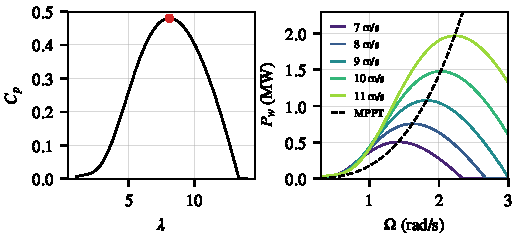
\includegraphics[width=0.8\textwidth]{turbine.pdf}
\caption{Power coefficient for $\beta=0$ (\textbf{left}) and captured power versus rotor speed with the
maximum power curve (\textbf{right}).}
\label{fig:turbine}
\end{figure}

\subsection{Electrical Modeling of the PMSG}
In the rotor $dq$ frame (amplitude-invariant transformation, $d$ axis aligned with the magnet flux),
with the receptor convention and $L_d=L_q=L_s$~\cite{aimene2022}, the stator voltages and the
electromagnetic torque are
\begin{align}
v_{sd} &= R_s i_{sd} + L_s\frac{di_{sd}}{dt} - \omega_e L_s i_{sq},\label{eq:vsd}\\
v_{sq} &= R_s i_{sq} + L_s\frac{di_{sq}}{dt} + \omega_e L_s i_{sd} + \omega_e\psi_f,\label{eq:vsq}\\
T_e &= \tfrac32 p\,\psi_f\, i_{sq},\label{eq:te}
\end{align}
where $\omega_e=p\Omega$ is the electrical speed, $p$ the number of pole pairs and $\psi_f$ the magnet
flux. In the receptor convention, $T_e<0$ and $i_{sq}<0$ in generating mode. With
$\bv{i}_s=[i_{sd}\;i_{sq}]^T$, $\bv{v}_s=[v_{sd}\;v_{sq}]^T$, $\bv{e}_q=[0\;1]^T$ and the
skew-symmetric matrix $\Jm=\bigl[\begin{smallmatrix}0&1\\-1&0\end{smallmatrix}\bigr]$,
(\ref{eq:vsd})--(\ref{eq:vsq}) are written in the compact form
\begin{equation}
L_s\dot{\bv{i}}_s = \bv{v}_s - R_s\bv{i}_s + \omega_eL_s\Jm\bv{i}_s - \omega_e\psi_f\bv{e}_q .
\label{eq:pmsg}
\end{equation}
The generator data are those of the non-salient 2~MW PMSG of~\cite{hasan2021}. At $\Omega_n$, the
back-electromotive force $p\Omega_n\psi_f=532$~V is close to the peak phase voltage of the grid (563~V).

\subsection{Mechanical Dynamics}
The direct-drive shaft is described by the one-mass model
\begin{equation}
J\frac{d\Omega}{dt} = T_w + T_e - B\Omega ,
\label{eq:shaft}
\end{equation}
where $J$ is the total inertia of the turbine and generator and $B$ the friction coefficient.

\subsection{Back-to-Back Converter and DC Link}
The two-level converters are represented by their average model, with voltage vectors limited to the
linear range $V_{dc}/\sqrt3$ of the space-vector modulation. The DC link receives the power of the MSC
and supplies the GSC~\cite{aimene2022}:
\begin{equation}
CV_{dc}\frac{dV_{dc}}{dt} = P_{dc} - P_i,\qquad P_{dc}=-\tfrac32\bv{v}_s^T\bv{i}_s,\qquad
P_i=\tfrac32\bv{v}_i^T\bv{i}_g ,
\label{eq:dc}
\end{equation}
where $\bv{v}_i$ is the GSC voltage and $\bv{i}_g$ the grid current.

\subsection{$L$ Filter and Grid}
In the grid-voltage-oriented frame ($v_{gq}=0$), with the current counted from the converter towards
the grid~\cite{aimene2022},
\begin{equation}
L_f\dot{\bv{i}}_g = \bv{v}_i - R_f\bv{i}_g + \omega_gL_f\Jm\bv{i}_g - \bv{v}_g ,
\label{eq:filter}
\end{equation}
where $\omega_g$ is the grid angular frequency, and the grid powers are $P_g=\frac32v_{gd}i_{gd}$ and
$Q_g=-\frac32v_{gd}i_{gq}$.

\subsection{Power Balance of the Model}
With the total stored energy
$E=\frac12J\Omega^2+\frac34L_s\|\bv{i}_s\|^2+\frac12CV_{dc}^2+\frac34L_f\|\bv{i}_g\|^2$, and since
$\bv{x}^T\Jm\bv{x}=0$ for any $\bv{x}$ and $T_e\Omega=\frac32\omega_e\psi_fi_{sq}$, the model
(\ref{eq:pw})--(\ref{eq:filter}) gives, for any state and any converter voltages,
\begin{equation}
\dot E = P_w - B\Omega^2 - \tfrac32R_s\|\bv{i}_s\|^2 - \tfrac32R_f\|\bv{i}_g\|^2 - P_g .
\label{eq:balance}
\end{equation}
The captured power is therefore stored, dissipated in the friction and in the resistances, or injected
into the grid. This balance verifies the sign of every term of the model; its numerical residual, evaluated
at random states and inputs, is below $10^{-15}P_n$.

\begin{table}[!htb]
\caption{Parameters of the studied system.}
\label{tab:param}
\centering
\begin{tabular}{llll}
\toprule
Parameter & Symbol & Value & Source\\
\midrule
Rated power & $P_n$ & 2 MW & \cite{hasan2021}\\
Rotor radius & $R$ & 40 m & \cite{rolan2009}\\
Air density & $\rho$ & 1.225 kg/m$^3$ & \cite{aimene2022}\\
Rated wind speed / rotor speed & $v_n$, $\Omega_n$ & 11.0 m/s, 2.23 rad/s & (\ref{eq:pw})\\
Total inertia & $J$ & $2.8\times10^6$ kg$\cdot$m$^2$ & assumed\\
Friction coefficient & $B$ & $10^3$ N$\cdot$m$\cdot$s & assumed\\
Pole pairs & $p$ & 26 & \cite{hasan2021}\\
Stator resistance & $R_s$ & 0.78 m$\Omega$ & \cite{hasan2021}\\
Stator inductance & $L_s$ & 1.57 mH & \cite{hasan2021}\\
Magnet flux & $\psi_f$ & 9.18 Wb & \cite{hasan2021}\\
DC-link capacitance and voltage & $C$, $V_{dc}^*$ & 20 mF, 1200 V & \cite{hasan2021}\\
Filter inductance and resistance & $L_f$, $R_f$ & 0.15 mH, 2 m$\Omega$ & \cite{hasan2021}, assumed\\
Grid voltage and frequency & & 690 V, 50 Hz & \cite{hasan2021}\\
Switching frequency & $f_{sw}$ & 2160 Hz & \cite{hasan2021}\\
\bottomrule
\end{tabular}
\end{table}

%=====================================================================
\section{Proposed Flatness-Based and Passivity-Based Control}
In this article, the outer loops are designed by differential flatness and the current loops by
passivity-based control. The objective of this combination is to compute the references directly from
the model, so that the generator power is passed to the grid without waiting for an error on the DC-link
voltage, while the current loops keep the energy structure of the machine and of the filter. The
architecture of the proposed control is presented in Figure~\ref{fig:structure}. All the errors are
defined as measured minus reference values. The controller is sampled at $T_s=1/(2f_{sw})=231.5~\mu$s,
and the converter voltages are applied one sample after their computation.

\begin{figure}[!htb]
\centering
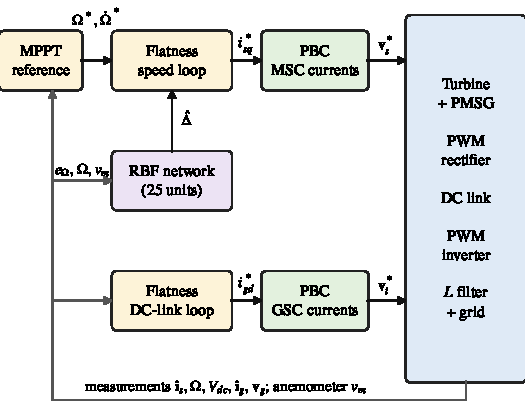
\includegraphics[width=0.7\textwidth]{structure.pdf}
\caption{Structure of the proposed control: flat outer loops, PBC current loops and adaptive RBF
compensation.}
\label{fig:structure}
\end{figure}

\subsection{MPPT Reference}
The optimal rotor speed $\Omega_{opt}=\lambda_{opt}v_m/R$, computed from the anemometer measurement $v_m$
and limited to $[0.5\Omega_n,\Omega_n]$, is filtered by the second-order model
\begin{equation}
\ddot\Omega^*=\omega_r^2(\Omega_{opt}-\Omega^*)-2\omega_r\dot\Omega^* ,
\label{eq:ref}
\end{equation}
with $\omega_r=1$~rad/s, which gives a smooth reference $\Omega^*$ and its derivative $\dot\Omega^*$.

\subsection{Flatness-Based Speed Loop}
From (\ref{eq:shaft}), $T_e=J\dot\Omega+B\Omega-T_w$: the rotor speed $\Omega$ is a flat output of the
shaft with input $T_e$, i.e., $i_{sq}$~\cite{fliess1995,aimene2022}. Imposing $\dot\Omega=\nu_1$ with
\begin{equation}
\nu_1=\dot\Omega^*-k_{11}e_\Omega-k_{12}\!\int\!e_\Omega\,dt,\qquad e_\Omega=\Omega-\Omega^*,
\end{equation}
gives the torque and current references
\begin{equation}
T_e^* = J\nu_1 + B\Omega - \hat T_w - \hat\Delta,\qquad i_{sq}^*=\frac{T_e^*}{\frac32p\psi_f},\qquad i_{sd}^*=0,
\label{eq:flat1}
\end{equation}
where $\hat T_w$ is computed from (\ref{eq:pw})--(\ref{eq:cp}) with $v_m$, and $\hat\Delta$ is the
neural compensation of Section~4 ($\hat\Delta=0$ for the nominal controller). $T_e^*$ is limited to
$[-1.2T_n,0]$, with the integration frozen at the limit. With $i_{sq}=i_{sq}^*$ and
$\Delta=T_w-\hat T_w$, the speed error obeys
\begin{equation}
J\bigl(\dot e_\Omega + k_{11}e_\Omega + k_{12}\!\textstyle\int\! e_\Omega\,dt\bigr) = \Delta-\hat\Delta .
\label{eq:errw}
\end{equation}

\subsection{Flatness-Based DC-Link Loop}
The flat output of the DC-link loop is the energy stored in the DC link and in the filter,
$y_2=\frac12CV_{dc}^2+\frac34L_f\|\bv{i}_g\|^2$. From (\ref{eq:dc})--(\ref{eq:filter}),
\begin{equation}
\dot y_2 = P_{dc} - P_g - \tfrac32R_f\|\bv{i}_g\|^2 ,
\label{eq:y2}
\end{equation}
which is linear in the grid power~\cite{thounthong2010}. Imposing $\dot y_2=-k_{21}e_y-k_{22}\int e_y\,dt$,
with $e_y=y_2-y_2^*$ and $y_2^*=\frac12CV_{dc}^{*2}+\frac34L_f\|\bv{i}_g^*\|^2$, gives
\begin{equation}
P_g^* = P_{dc} - \tfrac32R_f\|\bv{i}_g\|^2 + k_{21}e_y + k_{22}\!\int\! e_y\,dt,\qquad
i_{gd}^*=\frac{2P_g^*}{3v_{gd}},\qquad i_{gq}^*=0 ,
\label{eq:flat2}
\end{equation}
where $i_{gq}^*=0$ gives a unity power factor. $P_{dc}$ is computed from the applied MSC voltages and the
measured currents, so that the generator power is passed to the grid before it changes $V_{dc}$.

\subsection{Passivity-Based Current Loops}
With $\bv{e}_s=\bv{i}_s-\bv{i}_s^*$ and $\dot{\bv{z}}_s=\bv{e}_s$, the MSC voltage reference is
\begin{equation}
\bv{v}_s^* = L_s\dot{\bv{i}}_s^* + R_s\bv{i}_s^* - \omega_eL_s\Jm\bv{i}_s^* + \omega_e\psi_f\bv{e}_q
- R_a\bv{e}_s - K_i\bv{z}_s ,
\label{eq:pbc1}
\end{equation}
and, with $\bv{e}_g=\bv{i}_g-\bv{i}_g^*$ and $\dot{\bv{z}}_g=\bv{e}_g$, the GSC voltage reference is
\begin{equation}
\bv{v}_i^* = L_f\dot{\bv{i}}_g^* + R_f\bv{i}_g^* - \omega_gL_f\Jm\bv{i}_g^* + \bv{v}_g
- R_b\bv{e}_g - K_{ig}\bv{z}_g .
\label{eq:pbc2}
\end{equation}
The first terms of (\ref{eq:pbc1})--(\ref{eq:pbc2}) reproduce the desired dynamics with the workless
coupling terms, $R_a$ and $R_b$ inject damping, and the integral terms remove the steady-state errors.
The reference derivatives are obtained by first-order filters with a time constant of 2~ms, and the
integrals are frozen when the voltage reaches $V_{dc}/\sqrt3$.

\begin{theorem}
Consider the PMSG model (\ref{eq:pmsg}) with the control (\ref{eq:pbc1}) and $R_a,K_i>0$. The storage
function $H=\frac12L_s\|\bv{e}_s\|^2+\frac12K_i\|\bv{z}_s\|^2$ satisfies
$\dot H=-(R_s+R_a)\|\bv{e}_s\|^2\le0$, and $\bv{e}_s\to0$. The same result holds for the filter
(\ref{eq:filter}) with the control (\ref{eq:pbc2}).
\end{theorem}
\begin{proof}
Subtracting $L_s\dot{\bv{i}}_s^*$ from (\ref{eq:pmsg}) and inserting (\ref{eq:pbc1}) gives the error
dynamics
\begin{equation}
L_s\dot{\bv{e}}_s=-(R_s+R_a)\bv{e}_s+\omega_eL_s\Jm\bv{e}_s-K_i\bv{z}_s .
\end{equation}
Hence $\dot H=\bv{e}_s^TL_s\dot{\bv{e}}_s+K_i\bv{z}_s^T\bv{e}_s=-(R_s+R_a)\|\bv{e}_s\|^2$, since
$\bv{e}_s^T\Jm\bv{e}_s=0$. $H$ is therefore non-increasing and bounded, $\bv{e}_s$ and $\bv{z}_s$ are
bounded, and $\dot H$ is uniformly continuous. Barbalat's lemma~\cite{khalil2002} gives
$\bv{e}_s\to0$. The proof for (\ref{eq:filter}) and (\ref{eq:pbc2}) is identical, with $L_f$, $R_f+R_b$
and $K_{ig}$.
\end{proof}

The gains place double closed-loop poles: $k_{11}=2\omega_\Omega$, $k_{12}=\omega_\Omega^2$,
$k_{21}=2\omega_v$, $k_{22}=\omega_v^2$, $R_s+R_a=2\omega_iL_s$, $K_i=\omega_i^2L_s$,
$R_f+R_b=2\omega_iL_f$ and $K_{ig}=\omega_i^2L_f$. The bandwidths are separated by more than one decade
($\omega_\Omega=2$, $\omega_v=60$ and $\omega_i=500$~rad/s), so the inner loops can be considered fast
with respect to the outer ones (Table~\ref{tab:ctrl}).

%=====================================================================
\section{Adaptive RBF Neural Compensation}
Although the nominal controller makes the current errors converge, a residual speed error remains
because of the uncertainty $\Delta=T_w-\hat T_w$ in (\ref{eq:errw}). This uncertainty comes from the
$C_p$ model, from the anemometer, which measures the wind at one point and with a delay, and from the
generator parameters. Therefore, an RBF network is introduced as a complementary compensation
mechanism. The network does not replace the nominal controller; it generates the additional term
$\hat\Delta$ in the torque reference (\ref{eq:flat1}), and the gains $k_{11}$, $k_{21}$, $k_{22}$ and
those of the current loops are kept unchanged.

\subsection{ANN Input Vector}
The uncertainty $\Delta$ depends mainly on the operating point of the turbine, i.e., on the rotor speed
and on the wind speed. The input vector of the network is therefore
\begin{equation}
\bv{z}=\Bigl[\frac{\Omega}{\Omega_n}\;\;\frac{v_m}{v_n}\Bigr]^T ,
\label{eq:z}
\end{equation}
where the normalization by the rated values gives inputs of the order of one over the whole operating
region.

\subsection{RBF Structure and Compensation Signal}
On the operating region, the uncertainty is approximated by
\begin{equation}
\Delta=\bv{W}^{*T}\boldsymbol\phi(\bv{z})+\varepsilon,\qquad |\varepsilon|\le\bar\varepsilon ,
\label{eq:approx}
\end{equation}
where $\bv{W}^*$ is an ideal weight vector and $\varepsilon$ the approximation error~\cite{park1991}. The
network has 25 Gaussian functions
\begin{equation}
\phi_j(\bv{z})=\exp\Bigl(-\frac{\|\bv{z}-\bv{c}_j\|^2}{2b^2}\Bigr),\qquad j=1,\dots,25,
\label{eq:phi}
\end{equation}
centred on a $5\times5$ grid of $[0.5,1.1]^2$, with the width $b=0.15$. The compensation signal is
\begin{equation}
\hat\Delta=\hat{\bv{W}}^T\boldsymbol\phi(\bv{z}) ,
\label{eq:dh}
\end{equation}
where $\hat{\bv{W}}$ is the vector of the estimated weights. When the network is used, it replaces the
integral action of the speed loop ($k_{12}=0$): otherwise, the integral would absorb the slowly varying
part of $\Delta$ and the network would not learn it.

\subsection{Online Adaptive Law}
The weights are not trained offline; they are adapted online by the Lyapunov-based law
\begin{equation}
\dot{\hat{\bv{W}}} = \Gamma\bigl(\boldsymbol\phi(\bv{z})\,e_\Omega - \sigma\hat{\bv{W}}\bigr),\qquad
\hat{\bv{W}}(0)=0,
\label{eq:law}
\end{equation}
where $\Gamma>0$ is the adaptation gain and $\sigma>0$ the $\sigma$-modification~\cite{ioannou1996},
which limits the drift of the weights in the presence of noise and approximation error. The adaptation
is frozen when $T_e^*$ reaches its limit, so that the network does not learn the effect of the
saturation.

\subsection{Bounded Adaptive Compensation}
\begin{theorem}
Consider the speed error dynamics (\ref{eq:errw}) with $k_{12}=0$, the approximation (\ref{eq:approx}),
the compensation (\ref{eq:dh}) and the adaptive law (\ref{eq:law}) with $\Gamma,\sigma>0$, exact $J$ and
$B$, and no saturation. Then the speed error $e_\Omega$ and the weight error
$\tilde{\bv{W}}=\bv{W}^*-\hat{\bv{W}}$ are uniformly ultimately bounded.
\end{theorem}
\begin{proof}
With $k_{12}=0$, (\ref{eq:errw}) becomes
$J\dot e_\Omega=-Jk_{11}e_\Omega+\tilde{\bv{W}}^T\boldsymbol\phi+\varepsilon$. Consider the Lyapunov
function
\begin{equation}
V=\tfrac12Je_\Omega^2+\tfrac{1}{2\Gamma}\|\tilde{\bv{W}}\|^2 .
\end{equation}
Since $\dot{\tilde{\bv{W}}}=-\dot{\hat{\bv{W}}}$,
\begin{equation}
\dot V=-Jk_{11}e_\Omega^2+e_\Omega(\tilde{\bv{W}}^T\boldsymbol\phi+\varepsilon)
-\tfrac1\Gamma\tilde{\bv{W}}^T\dot{\hat{\bv{W}}}
=-Jk_{11}e_\Omega^2+e_\Omega\varepsilon+\sigma\tilde{\bv{W}}^T\hat{\bv{W}} .
\end{equation}
Using $\tilde{\bv{W}}^T\hat{\bv{W}}\le\frac12\|\bv{W}^*\|^2-\frac12\|\tilde{\bv{W}}\|^2$ and
$e_\Omega\varepsilon\le\frac{Jk_{11}}{2}e_\Omega^2+\frac{\bar\varepsilon^2}{2Jk_{11}}$ gives
\begin{equation}
\dot V\le-\frac{Jk_{11}}{2}e_\Omega^2-\frac\sigma2\|\tilde{\bv{W}}\|^2
+\frac{\bar\varepsilon^2}{2Jk_{11}}+\frac\sigma2\|\bv{W}^*\|^2 ,
\end{equation}
which is negative outside a compact set. Hence $e_\Omega$ and $\tilde{\bv{W}}$ are uniformly ultimately
bounded~\cite{khalil2002}.
\end{proof}

\begin{remark}
The size of the residual set decreases when $k_{11}$ increases and when $\sigma$ and $\bar\varepsilon$
decrease. Increasing $k_{11}$ would, however, amplify the measurement noise by $Jk_{11}$ in
(\ref{eq:flat1}); the network reduces the speed error without changing this gain.
\end{remark}

\begin{table}[!htb]
\caption{Controller, adaptive network and measurement parameters used in the simulations.}
\label{tab:ctrl}
\centering
\begin{tabular}{ll}
\toprule
Parameter & Value\\
\midrule
Speed loop (flat) & $\omega_\Omega=2$ rad/s: $k_{11}=4$, $k_{12}=4$ (0 with the network); $\omega_r=1$ rad/s\\
DC-link loop (flat) & $\omega_v=60$ rad/s: $k_{21}=120$, $k_{22}=3600$\\
PBC, MSC & $\omega_i=500$ rad/s: $R_a=1.57~\Omega$, $K_i=393~\Omega$/s\\
PBC, GSC & $\omega_i=500$ rad/s: $R_b=0.148~\Omega$, $K_{ig}=37.5~\Omega$/s\\
RBF network & 25 Gaussian units, $b=0.15$, inputs (\ref{eq:z})\\
Adaptation & $\Gamma=10^7$, $\sigma=0.02$ s$^{-1}$, $\hat{\bv{W}}(0)=0$\\
Sampling & $T_s=231.5~\mu$s, one-sample computation delay\\
Sensor noise (std) & currents 5 A, DC voltage 1 V, grid voltage 1 V, encoder speed 2 mrad/s\\
Measurement filters & speed 5 ms, $P_{dc}$ and $v_{gd}$ in (\ref{eq:flat2}) 2 ms, anemometer 1 s\\
\bottomrule
\end{tabular}
\end{table}

%=====================================================================
\section{Numerical Simulations}
This section presents the numerical results obtained with the proposed control. Two configurations are
compared in order to assess the contribution of the adaptive network: the nominal flatness-based and
passivity-based controller ($\hat\Delta=0$, with the integral action of the speed loop), and the same
controller with the RBF compensation. The gains of Table~\ref{tab:ctrl} are the same in both
configurations, so that any improvement can be attributed to the network.

The model is integrated with a fourth-order Runge--Kutta scheme at the step $T_s$ over 40~s, starting
from the maximum-power equilibrium. To obtain realistic results, the controller only uses measured
signals: white noise is added to the current, voltage and speed measurements, the encoder speed is
filtered, and the grid voltage contains background harmonics of order 5 (2\,\%, negative sequence) and
7 (1.5\,\%, positive sequence), i.e., a voltage distortion of 2.5\,\% (Table~\ref{tab:ctrl}).

Two wind profiles are applied (Figure~\ref{fig:wind}). The step profile (9~m/s, 11~m/s at 10~s and
8~m/s at 25~s), similar to the one of~\cite{aimene2022}, assesses the transient response. The turbulent
profile is
\begin{equation}
v(t) = V_{mean} + \sum_{k=1}^{3} A_k\sin(2\pi f_k t) + v_{turb}(t) ,
\label{eq:wind}
\end{equation}
with $V_{mean}=8.5$~m/s, $A=[1.5,\,0.2,\,0.3]$~m/s and $f=[0.03,\,0.16,\,0.17]$~Hz~\cite{regani2026}. The
turbulence $v_{turb}$ is a first-order coloured noise with a standard deviation of 0.5~m/s and a
correlation time of 1.5~s. Over 40~s, the turbulent wind remains between 6.0 and 10.9~m/s, below the rated
wind speed. The controller uses the anemometer measurement $v_m$, modeled by a first-order lag of 1~s.

\begin{figure}[!htb]
\centering
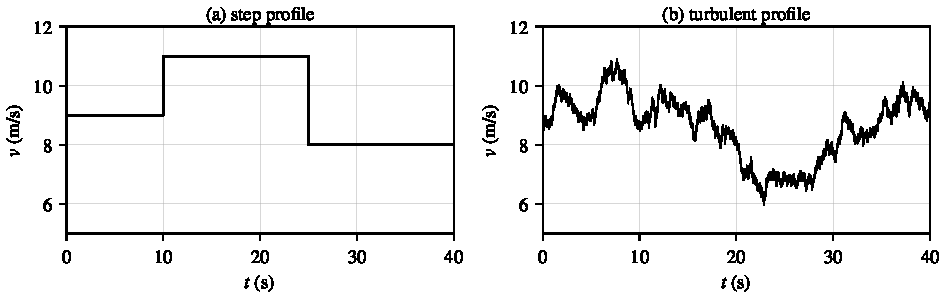
\includegraphics[width=\textwidth]{wind.pdf}
\caption{Applied wind-speed profiles: (\textbf{a}) step profile; (\textbf{b}) turbulent profile.}
\label{fig:wind}
\end{figure}

Three cases are considered: (i) step wind with nominal parameters; (ii) turbulent wind with nominal
parameters; (iii) robustness: turbulent wind, with a true plant that differs from the model of the
controller ($C_p\times1.1$, $J\times1.2$, $R_s\times1.5$, $L_s\times1.2$, $\psi_f\times0.95$,
$R_f\times1.5$, $L_f\times1.25$), and a 50\,\% grid voltage dip between 25 and 25.15~s.

The speed tracking performance is evaluated with the speed error $e_\Omega(t)=\Omega(t)-\Omega^*(t)$,
by the root-mean-square error, the mean absolute error, the maximum error, and the integral absolute and
squared errors:
\begin{equation}
\begin{gathered}
\mathrm{RMSE}=\sqrt{\frac1N\sum_{k=1}^Ne_\Omega^2(k)},\qquad
\mathrm{MAE}=\frac1N\sum_{k=1}^N|e_\Omega(k)|,\qquad
e_{\max}=\max_k|e_\Omega(k)|,\\
\mathrm{IAE}=\int|e_\Omega|\,dt,\qquad
\mathrm{ISE}=\int e_\Omega^2\,dt ,
\end{gathered}
\label{eq:metrics}
\end{equation}
computed from $t=1$~s to $t=40$~s.

\subsection{Step Wind}
Figure~\ref{fig:track} shows the references and the measured values of the controlled variables for
the step wind with the RBF compensation. The rotor speed follows the MPPT reference from 1.82 to 2.23
and then 1.62~rad/s. The currents $i_{sq}$ and $i_{gd}$ follow their references during the transients,
and $i_{sd}$ and $i_{gq}$ remain around zero, with the measurement noise and the 300~Hz ripple due to the
grid harmonics. The DC-link voltage stays within 7~V (0.6\,\%) of 1200~V, since the generator power is
passed to the grid through $P_{dc}$ in (\ref{eq:flat2}).

\begin{figure}[!htb]
\centering
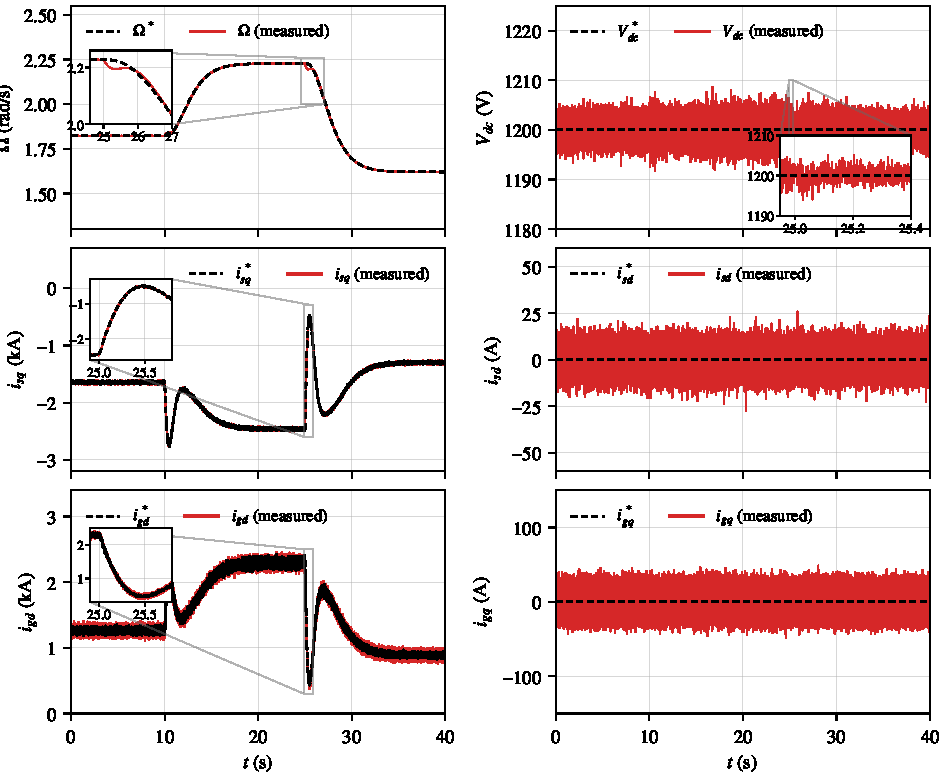
\includegraphics[width=\textwidth]{tracking_step.pdf}
\caption{Step wind, control with the RBF network: references (dashed) and measured values (solid) of the
rotor speed, DC-link voltage, and stator and grid currents, with enlarged views of the step at 25~s.}
\label{fig:track}
\end{figure}

\subsection{Turbulent Wind and Robustness}
Figure~\ref{fig:mppt} shows the robustness case with the RBF compensation. The rotor speed follows its
reference, and $C_p$ stays close to its maximum, except during the fast wind decrease around 22~s, where
the inertia prevents the rotor from slowing down quickly. The captured power follows the maximum available
power, and the difference between the captured and the injected powers corresponds to the kinetic energy
stored in or released by the rotor. The MPPT efficiency, i.e., the ratio between the captured energy and
the maximum available energy, is 97.7\,\%.

\begin{figure}[!htb]
\centering
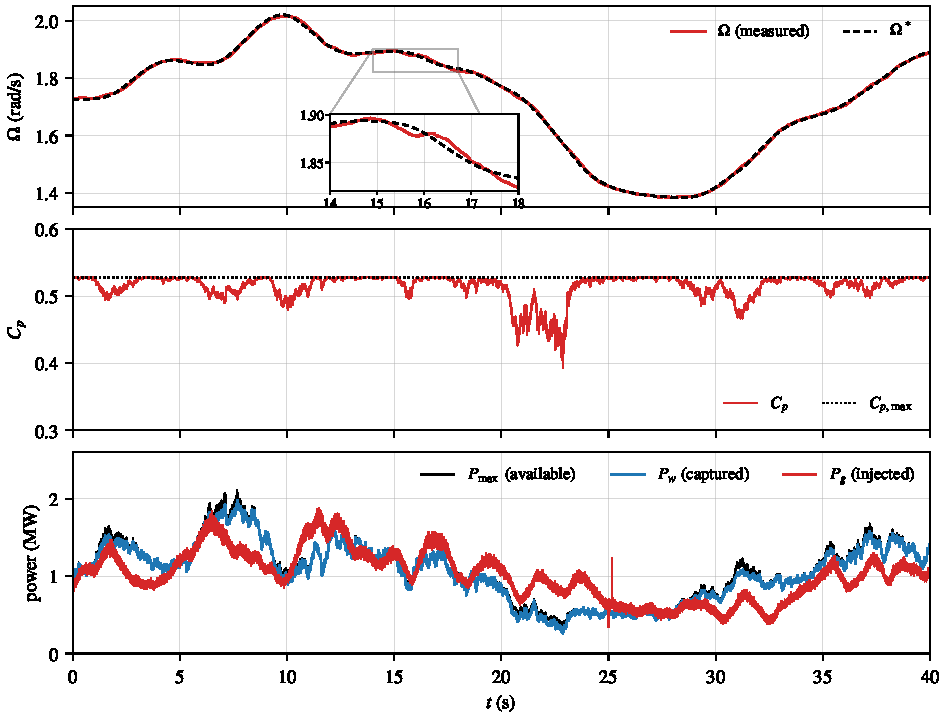
\includegraphics[width=\textwidth]{mppt.pdf}
\caption{Robustness case with the RBF network: rotor speed and reference, power coefficient (dotted:
$C_{p,\max}$ of the true turbine), and maximum available, captured and injected powers.}
\label{fig:mppt}
\end{figure}

\subsection{Effect of the Adaptive Neural Compensation}
Figure~\ref{fig:ann} compares the speed error without and with the network. For the step wind, the
error after each step vanishes in about 1.9~s with the network instead of 3.9~s without it. In the
turbulent cases, the error remains smaller, and the cumulative IAE grows more slowly over the whole
simulation. Figure~\ref{fig:net} shows that the network output follows the actual uncertainty; their
mean values are 82.5 and 83.4~kN$\cdot$m in the robustness case, i.e., about 14\,\% of the aerodynamic
torque.

\begin{figure}[!htb]
\centering
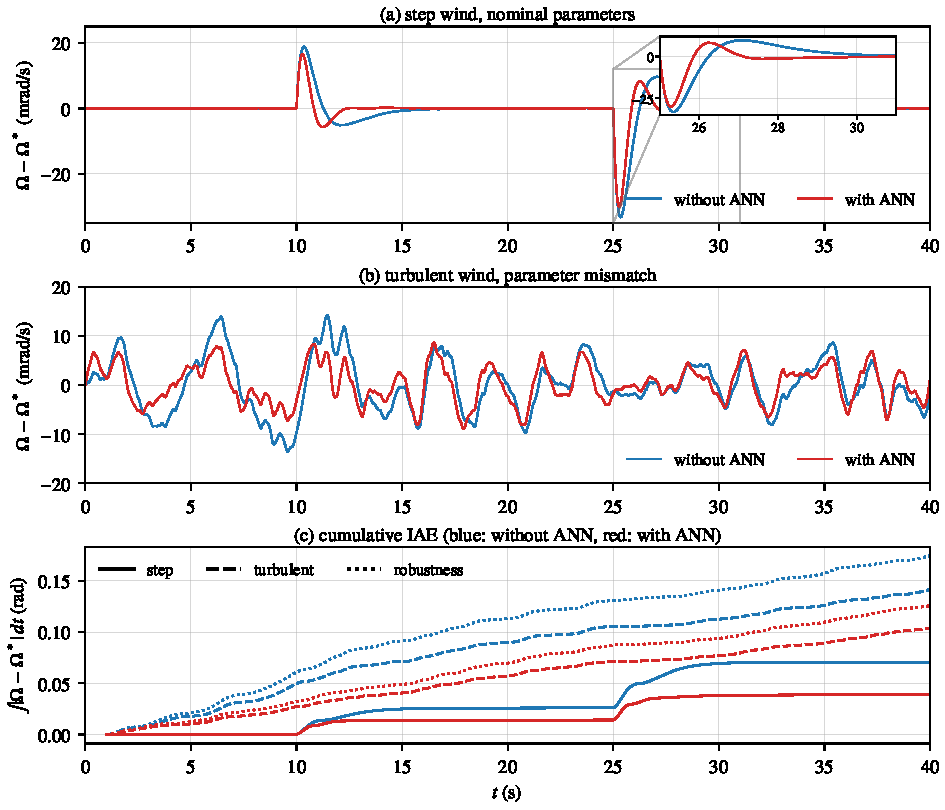
\includegraphics[width=\textwidth]{ann_effect.pdf}
\caption{Speed tracking error without and with the RBF network: (\textbf{a}) step wind, with an enlarged
view of the step at 25~s; (\textbf{b}) robustness case; (\textbf{c}) cumulative IAE for the three cases.}
\label{fig:ann}
\end{figure}

\begin{figure}[!htb]
\centering
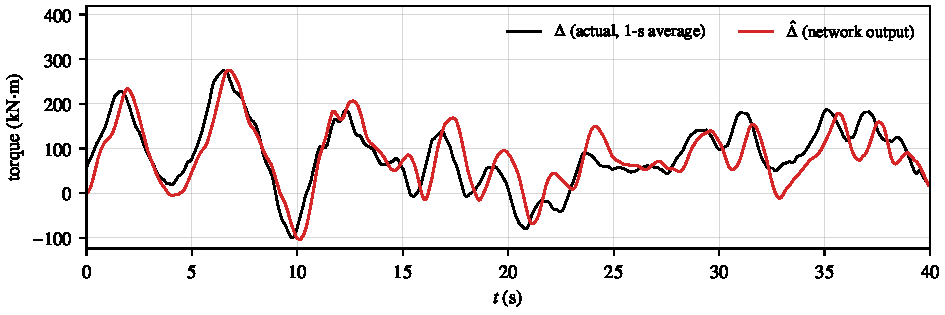
\includegraphics[width=\textwidth]{network.pdf}
\caption{Robustness case: output $\hat\Delta$ of the RBF network and actual uncertainty $\Delta$ (1-s
average).}
\label{fig:net}
\end{figure}

The speed tracking results are summarized in Table~\ref{tab:speed}. With the network, the IAE decreases
by 44.8\,\% for the step wind, 26.5\,\% for the turbulent wind and 27.9\,\% in the robustness case, and the
ISE decreases by 46 to 52\,\%, while the nominal gains remain unchanged. Table~\ref{tab:sys} shows that the
other variables are practically unchanged: the current errors, the DC-link deviation and the grid-current
distortion are the same, and the captured energy and the MPPT efficiency are equal. The grid-current total
harmonic distortion (THD), between 1.5 and 3.9\,\%, is below the 5\,\% limit of~\cite{ieee519}. The
price of the compensation is a slightly more active torque, with a 9 to 12\,\% larger standard deviation
of its rate.

\begin{table}[!htb]
\caption{Speed tracking performance of the nominal controller and of the controller with the adaptive RBF
compensation (best values in bold).}
\label{tab:speed}
\centering
\begin{tabular}{llccc}
\toprule
Case & Metric & Without ANN & With ANN & Improvement (\%)\\
\midrule
Step wind & RMSE (mrad/s) & 4.99 & \textbf{3.67} & 26.5\\
 & MAE (mrad/s) & 1.81 & \textbf{1.00} & 44.8\\
 & $e_{\max}$ (mrad/s) & 33.2 & \textbf{30.1} & 9.5\\
 & IAE (mrad) & 70.6 & \textbf{39.0} & 44.8\\
 & ISE ($10^{-4}$ rad$^2$/s) & 9.71 & \textbf{5.24} & 46.0\\
\midrule
Turbulent wind & RMSE (mrad/s) & 4.61 & \textbf{3.25} & 29.6\\
 & MAE (mrad/s) & 3.63 & \textbf{2.66} & 26.5\\
 & $e_{\max}$ (mrad/s) & 12.7 & \textbf{7.42} & 41.4\\
 & IAE (mrad) & 141.4 & \textbf{103.9} & 26.5\\
 & ISE ($10^{-4}$ rad$^2$/s) & 8.28 & \textbf{4.11} & 50.4\\
\midrule
Robustness & RMSE (mrad/s) & 5.55 & \textbf{3.87} & 30.4\\
 & MAE (mrad/s) & 4.47 & \textbf{3.22} & 27.9\\
 & $e_{\max}$ (mrad/s) & 14.2 & \textbf{8.93} & 37.0\\
 & IAE (mrad) & 174.3 & \textbf{125.7} & 27.9\\
 & ISE ($10^{-4}$ rad$^2$/s) & 12.0 & \textbf{5.83} & 51.5\\
\bottomrule
\end{tabular}
\end{table}

\begin{table}[!htb]
\caption{Performance of the whole system without and with the adaptive RBF compensation (40~s, from
$t=1$~s; best values in bold, both in bold when the difference is negligible).}
\label{tab:sys}
\centering
\small
\setlength{\tabcolsep}{4.5pt}
\begin{tabular}{lcccccc}
\toprule
 & \multicolumn{2}{c}{Step wind} & \multicolumn{2}{c}{Turbulent wind} & \multicolumn{2}{c}{Robustness}\\
\cmidrule(lr){2-3}\cmidrule(lr){4-5}\cmidrule(lr){6-7}
Metric & Without & With & Without & With & Without & With\\
\midrule
Max $|V_{dc}-V_{dc}^*|$ (V)$^{1}$ & \textbf{6.96} & \textbf{6.94} & \textbf{7.03} & \textbf{6.90} & \textbf{9.32} & \textbf{9.10}\\
RMS error of $i_{sq}$ (A) & \textbf{5.83} & \textbf{5.80} & \textbf{5.85} & \textbf{5.81} & \textbf{5.81} & \textbf{5.79}\\
RMS error of $i_{gd}$ (A) & \textbf{41.5} & \textbf{41.4} & \textbf{42.3} & \textbf{42.3} & \textbf{35.1} & \textbf{35.0}\\
Grid-current THD (\%) & \textbf{1.45} & \textbf{1.45} & \textbf{3.86} & \textbf{3.92} & \textbf{2.55} & \textbf{2.58}\\
Energy (kWh) & \textbf{13.86} & \textbf{13.86} & \textbf{10.05} & \textbf{10.04} & \textbf{10.98} & \textbf{10.97}\\
MPPT efficiency (\%) & \textbf{98.0} & \textbf{98.0} & \textbf{97.7} & \textbf{97.7} & \textbf{97.7} & \textbf{97.7}\\
Torque rate std (MN$\cdot$m/s)$^{2}$ & \textbf{0.239} & 0.267 & \textbf{0.212} & 0.231 & \textbf{0.210} & 0.233\\
\bottomrule
\end{tabular}

\vspace{2pt}{\footnotesize $^{1}$ outside the grid voltage dip; $^{2}$ of the torque averaged over 50~ms.}
\end{table}

\subsection{Grid Voltage Dip}
Figure~\ref{fig:grid} shows the 50\,\% voltage dip of the robustness case. The grid current doubles, from
0.8 to 1.6~kA, to keep the injected power, which remains below the current limit of the converter. The
DC-link voltage deviates by 16~V (1.3\,\%) at the beginning of the dip and returns within 5~V of 1200~V
about 50~ms after the end of the dip.

\begin{figure}[!htb]
\centering
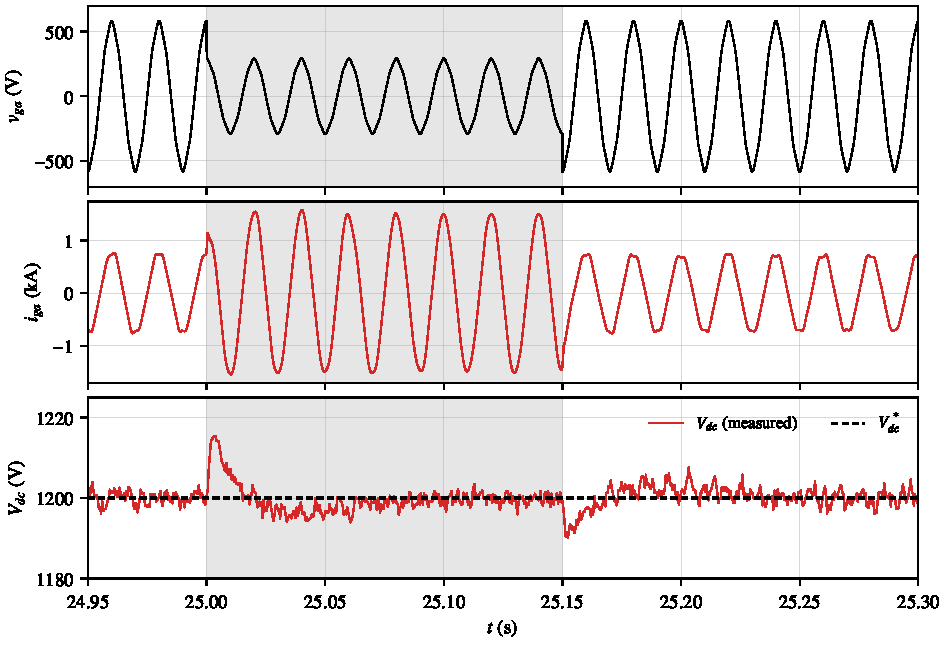
\includegraphics[width=\textwidth]{grid.pdf}
\caption{Robustness case: grid voltage and current of phase $a$ and DC-link voltage during the 50\,\%
voltage dip (shaded).}
\label{fig:grid}
\end{figure}

%=====================================================================
\section{Conclusions}
This paper presented a flatness-based and passivity-based control with adaptive RBF neural compensation
for a 2~MW direct-drive PMSG wind energy conversion system. The system was modeled from the wind to the
grid in the receptor convention, and an exact power balance verified the signs of the model. The rotor
speed and the energy of the DC link and of the filter were used as flat outputs, the currents of both
converters were controlled by PBC with a proof of convergence, and an RBF network adapted by a
Lyapunov-based law compensated the aerodynamic-torque and parameter uncertainty with uniformly ultimately
bounded errors. Simulation results with sensor noise, grid harmonics, parameter mismatch and a voltage dip
showed that all the controlled variables track their references, that the DC-link voltage remains within
0.8\,\% of its reference outside the dip, and that the network reduces the integral absolute speed error by
26.5 to 44.8\,\% with the same captured energy and the same nominal gains.

The proposed control has been validated by numerical simulations with the average model of the
converters, so the switching ripple is not represented, and with an ideal synchronization to the grid.
The turbulent wind was represented by one realization, and no experimental or hardware-in-the-loop (HIL)
validation has yet been performed. Moreover, the stability analysis assumes that the current loops are
fast with respect to the speed loop. These aspects will be addressed in future studies through a switching
model with an $LCL$ filter, the inclusion of the phase-locked loop dynamics, HIL implementation, and
comparative evaluations with other control strategies.

\vspace{10pt}
\noindent\small\textbf{Author Contributions:} Conceptualization, M.M. and K.K.; Methodology, S.R.;
Validation, S.R. and K.K.; Investigation, S.R.; Writing---original draft, S.R., M.M. and K.K.;
Supervision, M.M. and K.K.; Project administration, M.M. and K.K. All authors have read and agreed to the
published version of the manuscript.

\noindent\textbf{Funding:} This research received no external funding.

\noindent\textbf{Data Availability Statement:} The original contributions presented in this study are
included in the article. Further inquiries can be directed to the corresponding author.

\noindent\textbf{Conflicts of Interest:} The authors declare no conflicts of interest.
\normalsize

\begin{thebibliography}{99}
\small
\bibitem{barthelmie2021} Barthelmie, R.J.; Pryor, S.C. Climate Change Mitigation Potential of Wind Energy.
\emph{Climate} \textbf{2021}, \emph{9}, 136. https://doi.org/10.3390/cli9090136.
\bibitem{iea2024} International Energy Agency (IEA). \emph{World Energy Outlook 2024}; IEA: Paris, France, 2024.
\bibitem{gwec2024} Global Wind Energy Council (GWEC). \emph{Global Wind Report 2024}; GWEC: Brussels,
Belgium, 2024.
\bibitem{polinder2013} Polinder, H.; Ferreira, J.A.; Jensen, B.B.; Abrahamsen, A.B.; Atallah, K.;
McMahon, R.A. Trends in Wind Turbine Generator Systems. \emph{IEEE J. Emerg. Sel. Top. Power Electron.}
\textbf{2013}, \emph{1}, 174--185.
\bibitem{yaramasu2015} Yaramasu, V.; Wu, B.; Sen, P.C.; Kouro, S.; Narimani, M. High-Power Wind Energy
Conversion Systems: State-of-the-Art and Emerging Technologies. \emph{Proc. IEEE} \textbf{2015},
\emph{103}, 740--788.
\bibitem{wu2011} Wu, B.; Lang, Y.; Zargari, N.; Kouro, S. \emph{Power Conversion and Control of Wind
Energy Systems}; Wiley-IEEE Press: Hoboken, NJ, USA, 2011.
\bibitem{rolan2009} Rol\'an, A.; Luna, A.; V\'azquez, G.; Aguilar, D.; Azevedo, G. Modeling of a
Variable Speed Wind Turbine with a Permanent Magnet Synchronous Generator. In Proceedings of the IEEE
International Symposium on Industrial Electronics (ISIE), Seoul, Republic of Korea, 2009; pp.~734--739.
https://doi.org/10.1109/ISIE.2009.5218120.
\bibitem{hasan2021} Hasan, S.M.M.; Shatil, A.H.M. Design and Comparison of Grid Connected Permanent
Magnet Synchronous Generator Non-Salient Pole and Salient Pole Rotor Wind Turbine. \emph{AIUB J. Sci.
Eng.} \textbf{2021}, \emph{20}, 40--46.
\bibitem{chinchilla2006} Chinchilla, M.; Arnaltes, S.; Burgos, J.C. Control of Permanent-Magnet
Generators Applied to Variable-Speed Wind-Energy Systems Connected to the Grid. \emph{IEEE Trans. Energy
Convers.} \textbf{2006}, \emph{21}, 130--135.
\bibitem{yazdani2010} Yazdani, A.; Iravani, R. \emph{Voltage-Sourced Converters in Power Systems:
Modeling, Control, and Applications}; Wiley-IEEE Press: Hoboken, NJ, USA, 2010.
\bibitem{blaabjerg2006} Blaabjerg, F.; Teodorescu, R.; Liserre, M.; Timbus, A.V. Overview of Control and
Grid Synchronization for Distributed Power Generation Systems. \emph{IEEE Trans. Ind. Electron.}
\textbf{2006}, \emph{53}, 1398--1409.
\bibitem{mechter2015} Mechter, A.; Kemih, K.; Ghanes, M. Sliding Mode Control of a Wind Turbine with
Exponential Reaching Law. \emph{Acta Polytech. Hung.} \textbf{2015}, \emph{12}, 167--183.
\bibitem{mechter2016} Mechter, A.; Kemih, K.; Ghanes, M. Backstepping Control of a Wind Turbine for Low
Wind Speeds. \emph{Nonlinear Dyn.} \textbf{2016}, \emph{84}, 2435--2445.
https://doi.org/10.1007/s11071-016-2655-y.
\bibitem{messadi2015} Messadi, M.; Mellit, A.; Kemih, K.; Ghanes, M. Predictive Control of a Chaotic
Permanent Magnet Synchronous Generator in a Wind Turbine System. \emph{Chin. Phys. B} \textbf{2015},
\emph{24}, 010502.
\bibitem{yang2021} Yang, L.; Yang, F.; Sheng, W.; Zhou, K.; Huang, T. Fuzzy Chaos Control of Fractional
Order D-PMSG for Wind Turbine with Uncertain Parameters by State Feedback Design. \emph{Energies}
\textbf{2021}, \emph{14}, 7369.
\bibitem{benabdeeseelam2025} Benabdeeseelam, A.; Messadi, M.; Kemih, K.; Hamiche, H. Chattering-Free
Terminal Sliding Mode Control Based on Adaptive Exponential Reaching Barrier Function for a Chaotic
Permanent Magnet Synchronous Generator in Offshore Wind Turbine System. \emph{Chin. Phys. B}
\textbf{2025}, \emph{34}, 090501.
\bibitem{fliess1995} Fliess, M.; L\'evine, J.; Martin, P.; Rouchon, P. Flatness and Defect of Non-Linear
Systems: Introductory Theory and Examples. \emph{Int. J. Control} \textbf{1995}, \emph{61}, 1327--1361.
\bibitem{aimene2022} Aimene, M.; Payman, A.; Dakyo, B. Comparative Study between Flatness-Based and
Field-Oriented Control Methods of a Grid-Connected Wind Energy Conversion System. \emph{Processes}
\textbf{2022}, \emph{10}, 378. https://doi.org/10.3390/pr10020378.
\bibitem{thounthong2010} Thounthong, P.; Pierfederici, S.; Davat, B. Analysis of Differential
Flatness-Based Control for a Fuel Cell Hybrid Power Source. \emph{IEEE Trans. Energy Convers.}
\textbf{2010}, \emph{25}, 909--920.
\bibitem{ortega1998} Ortega, R.; Lor\'ia, A.; Nicklasson, P.J.; Sira-Ram\'irez, H.
\emph{Passivity-Based Control of Euler-Lagrange Systems}; Springer: London, UK, 1998.
\bibitem{ortega2002} Ortega, R.; van der Schaft, A.; Maschke, B.; Escobar, G. Interconnection and
Damping Assignment Passivity-Based Control of Port-Controlled Hamiltonian Systems. \emph{Automatica}
\textbf{2002}, \emph{38}, 585--596.
\bibitem{park1991} Park, J.; Sandberg, I.W. Universal Approximation Using Radial-Basis-Function
Networks. \emph{Neural Comput.} \textbf{1991}, \emph{3}, 246--257.
\bibitem{lewis1999} Lewis, F.L.; Jagannathan, S.; Ye\c{s}ildirek, A. \emph{Neural Network Control of
Robot Manipulators and Nonlinear Systems}; Taylor \& Francis: London, UK, 1999.
\bibitem{li2024} Li, Y.; Sun, W.; Yu, D. RBFNN-Based Global Fast Terminal Sliding Mode Control for Fully
Controlled Doubly Fed Induction Generator. \emph{J. Frankl. Inst.} \textbf{2024}, \emph{361}, 107196.
https://doi.org/10.1016/j.jfranklin.2024.107196.
\bibitem{dardabi2024} Dardabi, C.; Djebli, A.; Chojaa, H. Enhancing the Control of Doubly Fed Induction
Generators Using Artificial Neural Networks in the Presence of Real Wind Profiles. \emph{PLoS ONE}
\textbf{2024}, \emph{19}, e0300527. https://doi.org/10.1371/journal.pone.0300527.
\bibitem{bounar2025} Bounar, N.; Boulkroune, A.; Labdai, S.; Chrifi-Alaoui, L.; Khebbache, H.
Disturbance Observer-Based Finite-Time Adaptive Neural Control Scheme of DFIG-Wind Turbine. \emph{Wind
Eng.} \textbf{2025}, \emph{49}, 271--289. https://doi.org/10.1177/0309524X241263517.
\bibitem{regani2026} Regani, S.; Messadi, M.; Kemih, K. A Novel Chaos Control Approach with Adaptive ANN
Compensation for a DFIG-Based Wind Turbine. \emph{Mathematics} \textbf{2026}, \emph{14}, 3739.
https://doi.org/10.3390/math14203739.
\bibitem{heier2014} Heier, S. \emph{Grid Integration of Wind Energy: Onshore and Offshore Conversion
Systems}, 3rd ed.; Wiley: Chichester, UK, 2014.
\bibitem{khalil2002} Khalil, H.K. \emph{Nonlinear Systems}, 3rd ed.; Prentice Hall: Upper Saddle River,
NJ, USA, 2002.
\bibitem{ioannou1996} Ioannou, P.A.; Sun, J. \emph{Robust Adaptive Control}; Prentice Hall: Upper Saddle
River, NJ, USA, 1996.
\bibitem{ieee519} \emph{IEEE Std 519-2014}; IEEE Recommended Practice and Requirements for Harmonic
Control in Electric Power Systems. IEEE: New York, NY, USA, 2014.
\end{thebibliography}

\end{document}
